\documentclass[english]{article}
\usepackage{tikz}
\usepackage{pgfplots}
\pgfplotsset{compat=1.10}
\usetikzlibrary{shapes.geometric,arrows,fit,matrix,positioning}
\tikzset
{
    treenode/.style = {circle, draw=black, align=center, minimum size=1cm},
    subtree/.style  = {isosceles triangle, draw=black, align=center, minimum height=0.5cm, minimum width=1cm, shape border rotate=90, anchor=north}
}
\usepackage[letterpaper]{geometry}
\geometry{verbose,tmargin=1in,bmargin=1in,lmargin=1in,rmargin=1in}
\usepackage{babel}
\usepackage{amsmath}
\usepackage{amssymb}
\usepackage{capt-of}
\usepackage{graphicx}
\usepackage{color}
\usepackage{latexsym}
\usepackage{xspace}
\usepackage{pdflscape}
\usepackage[hyphens]{url}
\usepackage[colorlinks]{hyperref}
\usepackage{enumerate}
\usepackage{ifthen}
\usepackage{float}
\usepackage{array}
\usepackage{tikz}
\usepackage{multirow} 
\usetikzlibrary{shapes}
\usepackage{algorithm2e}
\usepackage{listings}
\usepackage{diagbox}
\usepackage{tikz}

%%%% CUSTOM MATH GOES HERE
\newcommand{\ind}[1]{\mathbf{1}\left(#1\right)}
\renewcommand{\Pr}{\mathbf{Pr}\xspace}
\newcommand{\Bern}{\textsf{Bernoulli}\xspace}
\newcommand{\sign}{\textsf{sign}}
\newcommand{\E}{\mathbf{E}}
\newcommand{\bx}{\mathbf{x}}
\newcommand{\bX}{\mathbf{X}}
\newcommand{\by}{\mathbf{y}}
\newcommand{\bY}{\mathbf{Y}}
\newcommand{\bz}{\mathbf{z}}
\newcommand{\bw}{\mathbf{w}}
\newcommand{\bl}{\mathbf{\ell}}
\newcommand{\vc}[1]{\mathbf{#1}}
\newcommand{\Hypo}{\mathcal{H}}
\newcommand{\XX}{\mathcal{X}}
\newcommand{\cD}{\mathcal{D}}
\newcommand{\argmax}{\operatornamewithlimits{argmax}}
\newcommand{\argmin}{\operatornamewithlimits{argmin}}
\newcolumntype{M}{>{$\vcenter\bgroup\hbox\bgroup}c<{\egroup\egroup$}}
\newcolumntype{x}[1]{>{\centering\arraybackslash}m{#1}}

%%%%%%%%%%%%%%%%%%%%%%%%%%%%%%%%%

\title{CIS 520, Machine Learning, Fall 2018: Assignment 7\\}
\date{}
\author{Wentao He}

\begin{document}
\maketitle
{\normalsize Collaborator: \underline{N/A}}

\section{Hidden Markov Models}
\begin{enumerate}
    \item $P(X_{1:2} = (\text{sing}, \text{TV}), Z_{1:2} = (\text{happy}, \text{happy}))$
    \begin{align*}
    = &\; P(Z_1 = \text{happy})P(Z_2 = \text{happy}|Z_1=\text{happy})P(X_1 = \text{sing}|Z_1 = \text{happy})P(X_2 = \text{TV}|Z_2=\text{happy})\\
    = &\; \dfrac{1}{2} \times \dfrac{4}{5} \times \dfrac{5}{10} \times \dfrac{2}{10}\\
    = &\; \dfrac{16}{400}
    \end{align*}
    \item $P(X_{1:2} = (\text{sing}, \text{TV}), Z_{1:2} = (\text{happy}, sad))$
    \begin{align*}
    = &\; P(Z_1 = \text{happy})P(Z_2 = \text{sad}|Z_1=\text{happy})P(X_1 = \text{sing}|Z_1 = \text{happy})P(X_2 = \text{TV}|Z_2=\text{sad})\\
    = &\; \dfrac{1}{2} \times \dfrac{1}{5} \times \dfrac{5}{10} \times \dfrac{7}{10}\\
    = &\; \dfrac{14}{400}
    \end{align*}
    \item $P(X_{1:2} = (\text{sing}, \text{TV}), Z_{1:2} = (sad, \text{happy}))$
    \begin{align*}
    = &\; P(Z_1 = \text{sad})P(Z_2 = \text{happy}|Z_1=\text{sad})P(X_1 = \text{sing}|Z_1 = \text{sad})P(X_2 = \text{TV}|Z_2=\text{happy})\\
    = &\; \dfrac{1}{2} \times \dfrac{1}{2} \times \dfrac{1}{10} \times \dfrac{2}{10}\\
    = &\; \dfrac{2}{400}
    \end{align*}
    \item $P(X_{1:2} = (\text{sing}, \text{TV}), Z_{1:2} = (sad, sad))$
    \begin{align*}
    = &\; P(Z_1 = \text{sad})P(Z_2 = \text{sad}|Z_1=\text{sad})P(X_1 = \text{sing}|Z_1 = \text{sad})P(X_2 = \text{TV}|Z_2=\text{sad})\\
    = &\; \dfrac{1}{2} \times \dfrac{1}{2} \times \dfrac{1}{10} \times \dfrac{7}{10}\\
    = &\; \dfrac{7}{400}
    \end{align*}
    The most likely hidden state sequence $z_{1:2}$ is $z_{1:2}=(\text{happy},\text{happy})$. \\\\For individual mostly likely hidden state on day 2 is:
    \begin{align*}
    P&\;(X_{1:2} = (\text{sing}, \text{TV}), Z_2 = \text{happy})\\
    &\; = P(X_{1:2} = (\text{sing}, \text{TV}), Z_{1:2} = (\text{happy}, \text{happy})) + P(X_{1:2} = (\text{sing}, \text{TV}), Z_{1:2} = (\text{sad}, \text{happy}))\\
    &\; = \dfrac{16}{400} + \dfrac{2}{400}\\
    &\; = \dfrac{18}{400}\\\\
    P&\;(X_{1:2} = (\text{sing}, \text{TV}), Z_2 = \text{sad})\\
    &\; = P(X_{1:2} = (\text{sing}, \text{TV}), Z_{1:2} = (\text{happy}, \text{sad})) + P(X_{1:2} = (\text{sing}, \text{TV}), Z_{1:2} = (\text{sad}, \text{sad}))\\
    &\; = \dfrac{14}{400} + \dfrac{7}{400}\\
    &\; = \dfrac{21}{400}
    \end{align*}
    Therefore the individually most likely hidden state on day 2 is sad.
\end{enumerate}
\clearpage
\section{Mis\text{sing} Data}
\begin{enumerate}
    \item 0.9600
    \item With mean: 0.9200. Add an additional column: 0.8667.
    \item With mean: 0.9333. Add an additional column: 0.9467.
    \item Adding an indicator will lower the accuracy compared to imputing by means when it comes to random missing data. It is because that adding an indicator for random missing data isn't equal to adding an useful feature. Due to the fact that the data that is missing is random, if we merely the indicator (either 0 or 1) to represent the real data, it will introduce more error. However, when only 20\% of the data is missing and the missing ones are not random, adding an indicator will become actually useful. So adding an indicator works better in non-random cases.
\end{enumerate}
\clearpage
\section{Bayesian Networks}
\begin{enumerate}
    \item $p(x_1, x_2, x_3, x_4, x_5, x_6) = p(x_1)p(x_2)p(x_3|x_1, x_2)p(x_4|x_2)p(x_5|x_3)p(x_6|x_3, x_4)$
    \item $p(x_1, x_2, x_3, x_4, x_5, x_6) = p(x_1)p(x_2)p(x_3)p(x_4)p(x_5|x_3)p(x_6|x_3)$ This distribution included in the class of joint probability distribution can be represented by the Bayesian network above. It satisfies all the conditional independence assumptions implied. Some conditional probability are simply redundant.
    \item The class of joint probability distributions will be smaller becasue removing an edge will have the same effect as introducing an additional conditional independence assumption, which will then reduce the class of probability distributions.
    \item Given the above figure, determine whether each of the following is true or false. Briefly justify your answer.
    \begin{enumerate}
        \item \textbf{False}. Given $x_2$, $x_3$ and $x_4$ are conditionally independent, not unconditionally independent.
        \item \textbf{True}. If we perform Bayes ball algorithm starting at $x_1$, we would observe that there is no path that is able to reach $x_4$ since both $x_3$ and $x_6$ are unobserved. Therefore $x_1$ and $x_4$ are d-separated, which means independent.
        \item \textbf{False}. $x_6$ is a descendant of $x_3$. The observation of $x_6$ means that $x_1$ and $x_2$ are conditionally dependent.
        \item \textbf{False}. If we perform Bayes ball algorithm starting at $x_1$, the path from $x_1 \Rightarrow x_3 \Rightarrow x_6$ will be blocked because of the observation of $x_3$. However, we are still able to reach $x_6$ following the path $x_1 \Rightarrow x_3 \Rightarrow x_2 \Rightarrow x_4 \Rightarrow x_6$. Therefore $x_1$ and $x_6$ are not d-separated by $x_3$, which means both $x_1$ and $x_6$ are conditionally dependent given $x_3$.
    \end{enumerate}
\end{enumerate}
\clearpage
\section{Belief Net Construction}
\begin{enumerate}
    \item \textbf{A}\\\\
    Since A is the first variable, it doesn't have any parents. It's just A itself.
    \item \textbf{B}\\\\
    $P(B|A)=0.53, P(B|\sim A)=0.57, P(B)=0545$. Thus $|P(B|A)P(B)|<0.05, P(B|\sim )<0.05$. Neither equality test fails, therefore is no link from A to B.
    \item \textbf{C}\\\\
    When $A=T, B=T, P(C=T)=0.5$.\\
    When $A=T, B=F, P(C=T)=0.86$.\\
    When $A=F, B=T, P(C=T)=0.75$.\\
    When $A=F, B=F, P(C=T)=0.67$.\\\\
    We then get $P(C)=0.68$, and the range $P(C|\pm A, \pm B)| = 8.86-0.5>0..05$. Therefore C depends on the joint distribution of A and B and we need to add one link from A to C and one from B to C. Also we need to check whether these two links are redundant.\\\\
    The link from B to C:\\
    $|P(C|A,B)-P(C|A,\sim B)| = |0.5-0.86|>>0.05$, so we keep the link.\\\\
    The link from A to C:\\
    $|P(C|A,B)-P(C|\sim A, B)| = |0.5-0.75|>0.05$, so we keep the link.\\\\
    The above shows that C depends on both A and B. Therefore A and B both have link to C.
    \item \textbf{D}\\\\
    When $A=T, B=T, C=T, P(D=T)=0.75$.\\
    When $A=F, B=T, C=T, P(D=T)=0.33$.\\
    When $A=T, B=F, C=T, P(D=T)=0.33$.\\
    When $A=T, B=T, C=F, P(D=T)=0$.\\
    When $A=F, B=F, C=T, P(D=T)=0.5$.\\
    When $A=F, B=T, C=F, P(D=T)=0$.\\
    When $A=T, B=F, C=F, P(D=T)=0$.\\
    When $A=F, B=F, C=F, P(D=T)=0$.\\\\
    Thte range $|P(D|\pm A, \pm B, \pm C)| = 0.75 > 0.05$. Therefore D depends on the joint distribution of A, B and C, and we need to add one link from A to D, one from B to D and one from C to D. Also we need to check whether these three links are redundant.\\\\
    The link from A to D:\\
    $|P(D|A, \sim B, C)-P(D|\sim A,\sim B,C)|=|0.33-0.5|>0.05$, so we keep the link.\\\\
    The link from B to D:\\
    $|P(D|A, B, C)-P(D|A,\sim B,C)|=|0.75-0.33|>0.05$, so we keep the link.\\\\
    The link from C to D:\\
    $|P(D|A, B, C)-P(D|A,B,\sim C)|=|0.75-0|>0.05$, so we keep the link.\\\\
    The final Bayes net is:
\begin{center}
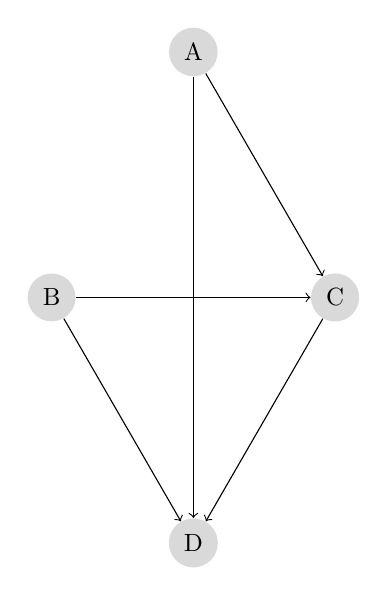
\begin{tikzpicture}[scale=.9, transform shape]
\tikzstyle{every node} = [circle, fill=gray!30]
\node (a) at (0, 0) {B};
\node (b) at +(0: 4) {C};
\node (c) at +(60: 4) {A};
\node (d) at +(-60: 4) {D};
\foreach \from/\to in {c/b, c/d, a/b, a/d, b/d}
\draw [->] (\from) -- (\to);
\end{tikzpicture}
\end{center}
\end{enumerate}
\clearpage
\section{EM}
\begin{enumerate}
    \item Based on the dependencies of the belief net, we are able to write the following probability: $P(A, B, C, D) = P(A)P(B)P(C|A,B)P(D|C)$. Therefore, the following parameters need to be learned: $P(A=T), P(B=T), P(C = T | A = T,B = T), P(C = T | A = F,B = T), P(C = T | A = T,B = F), P(C = T | A = F,B = F), P(D = T | C = T), P(D = T | C = F)$. We can use $\theta$ to represent the collection of these parameters. Since C is hidden, it means the values of $C_i$ is hidden and i represent the observations for $i = 1, \cdots, n$. Here $C_i$ is the random variable that represents C's value (either True or False) when it's the $i$-th observation. So the model is $p(z, x|\theta) = p(A)p(B)p(C = z | A, B)p(D | C = z)$. Here, $A, B, and D$ are observed in $x$ and $z$ is the hidden possible values (either True or False) of C for x. Before we initialize E-M, those parameters should be set to some value like $\frac{1}{2}$ and other numbers suitable for a probability.
    \item $p(C_i = z | x_i, \theta^{t-1}) = \dfrac{P(C_i = z, x_i | \theta^{t-1})}{P(C_i =T, x_i |\theta^{t-1} + P(C_i =F, x_i |\theta^{t-1})}$
    \item
    \begin{align*}
    \theta_t = &\; \argmax_\theta F(a^t, \theta)\\
    &\; = \argmax_\theta \sum_i \sum_z q^t(Z_i = z|x_i)\log p(z,x_i|\theta)\\
    &\; = \argmax_\theta \sum_i \sum_{z=T, F} p(C_i = z|x_i, \theta^{t-1})\log [p(A)p(B)p(C=Z|A,B)p(D|C=z)]\\
    &\; \textrm{From the E step, the equation can be written as:}\\
    &\; = \argmax_\theta \sum_i \sum_{z=T, F} \dfrac{P(C_i = z, x_i | \theta^{t-1})}{P(C_i =T, x_i |\theta^{t-1} + P(C_i =F, x_i |\theta^{t-1})} \log [p(A)p(B)p(C=Z|A,B)p(D|C=z)])
    \end{align*}
    \item Give the equations for the E and M steps for this case.
    \begin{enumerate}
        \item For the E step:\\
        \begin{enumerate}
            \item When C is missing:\\\\
            $p(C_i = z | x_i, \theta^{t-1}) = \dfrac{P(C_i = z, x_i | \theta^{t-1})}{P(C_i =T, x_i |\theta^{t-1} + P(C_i =F, x_i |\theta^{t-1})}$\\
            \item When D is missing:\\\\
            $p(D_i = z | x_i, \theta^{t-1}) = \dfrac{P(D_i = z, x_i | \theta^{t-1})}{P(D_i =T, x_i |\theta^{t-1} + P(D_i =F, x_i |\theta^{t-1})}$\\
            \item When both C and D are missing:\\\\
            $p(C_i = z_1, D_i = z_2 | x_i, \theta^{t-1}) = \dfrac{P(C_i = z_1, D_i = z_2, x_i | \theta^{t-1})}{P(C_i = T, D_i = T, x_i|\theta^{t-1})+\cdots+P(C_i = F, D_i = F, x_i|\theta^{t-1})}$\\\\
            The full expression of the demoninator is $P(C_i = T, D_i = T, x_i|\theta^{t-1})+P(C_i = T, D_i = F, x_i|\theta^{t-1})+P(C_i = F, D_i = T, x_i|\theta^{t-1})+P(C_i = F, D_i = F, x_i|\theta^{t-1})$.
        \end{enumerate}
        \item For the M step:\\
        \begin{align*}
        \theta_t = &\; \argmax_\theta F(a^t, \theta)\\
    &\; = \argmax_\theta \sum_i \sum_z q^t(Z_i = z|x_i)\log p(z,x_i|\theta)\\
    &\; = \argmax_\theta \sum_{i=0}^{n/2} \sum_{z=T, F} p(C_i = z|x_i, \theta^{t-1})\log [p(A)p(B)p(C=Z|A,B)p(D|C=z)],\\
    &\; +  \sum_{i=n/2}^{3n/4} \sum_{z=T, F} p(D_i = z|x_i, \theta^{t-1})\log [p(A)p(B)p(C|A,B)p(D=z|C)],\\
    &\; +  \sum_{i=3n/4}^{n} \sum_{z_1=T, F} \sum_{z_2 = T, F} p(C_i = z_1, D_i = z_2 |x_i, \theta^{t-1})\log [p(A)p(B)p(C=z_1|A,B)p(D=z_2 | C=z_1)] \\
    &\; \textrm{From the E step, the equation can be written as:}\\
    &\; = \argmax_\theta \sum_{i=0}^{n/2} \sum_{z=T, F} \dfrac{P(C_i = z, x_i | \theta^{t-1})}{P(C_i =T, x_i |\theta^{t-1} + P(C_i =F, x_i |\theta^{t-1})} \log [p(A)p(B)p(C=Z|A,B)p(D|C=z)]\\
    &\; + \sum_{i=n/2}^{3n/4} \sum_{z=T, F} \dfrac{P(D_i = z, x_i | \theta^{t-1})}{P(D_i =T, x_i |\theta^{t-1} + P(D_i =F, x_i |\theta^{t-1})} \log [p(A)p(B)p(C|A,B)p(D=z|C)]\\
    &\; + \sum_{i=3n/4}^{n} \sum_{z_1=T, F} \sum_{z_2 = T, F} \dfrac{P(C_i = z_1, D_i = z_2, x_i | \theta^{t-1})}{P(C_i = T, D_i = T, x_i|\theta^{t-1})+\cdots+P(C_i = F, D_i = F, x_i|\theta^{t-1})}
        \end{align*}
        The full expression of the demoninator of the last term for the above equation is $P(C_i = T, D_i = T, x_i|\theta^{t-1})+P(C_i = T, D_i = F, x_i|\theta^{t-1})+P(C_i = F, D_i = T, x_i|\theta^{t-1})+P(C_i = F, D_i = F, x_i|\theta^{t-1})$.
    \end{enumerate}
\end{enumerate}

\end{document}